% 
% File:    chapter-prediction.tex
% Author:  awl8049
% Revision:$Revision: 2.1 $
%
\chapter{Effective Prediction}
\label{chp:application}
The current generation of server systems lacks (1)~the complete set of
measurement and monitoring capabilities and (2)~data flow state capture
mechanisms required in order to formulate the parameters of an exact
analytical model.  For example, the system board DC and AC power
consumption cannot be easily split in measurements or analyses, due to
the presence of large numbers of voltage/current domains, each with
multiple components.  Therefore, effective prediction on future power
consumption based on past power consumption readings/measurements
(obtained from PeCs and performance metrics) is critical.

In \equationname~\eqref{eq:linmodel}, $E_{system}$ signifies total
energy consumed by the system for a given computational workload, equal
to the sum of five terms: $E_{proc}$, $E_{mem}$, $E_{hdd}$, $E_{board}$,
and $E_{em}$.  Adopting \equationname~\eqref{eq:linmodel} for server
energy consumption estimation, one needs to predict change in
$E_{system}$ over the time interval of $(t, t+\Delta t)$.  Such
prediction, following a time series to make observations of the server
system, based on PeCs and performance metrics, can be approximated by
\begin{equation}
\label{eq:tseries}
E_{system} = \hat{f}(E_{proc}, E_{mem}, E_{hdd}, E_{board}, E_{em}),
\end{equation}
where the involved parameters correspond to the five server energy
contributors modeled in Sections~\ref{sec:procmodel} to
\ref{sec:electrical}. Similar time series are created for the quantities
defined $Theta(A,D_{A},t)$ and $C_{theta}(A,D_{A},T,t)$ for use in
thermal prediction, with parameters also taken from the five server
energy contributors defined in Sections~\ref{sec:procmodel} to
\ref{sec:electrical}.

\section{Performance counters and metrics}
\label{sec:variables}
In our prediction approach, fourteen (14) observable PeCs and accessible
performance metrics (referred to as "measures" collectively for simplicity)
are involved in the AMD server, as listed in Table~\ref{tab:model}.
They are grouped into five clusters, depending on their relevance to the
server energy contributors.  More specifically, the top three measures
are related to $E_{proc}$, named $MP_{proc}^{AMD} = \left[T_{C_{0}},
  T_{C_{1}}, HT_{1}\right]$.  The next five measures dictate $E_{mem}$,
denoted by $MP_{mem}^{AMD} = \left[HT_{2}, CM_{0}, CM_{1}, CM_{2},
  CM_{3}\right]$.  Those $CM_i$ measures, capturing the total L2 cache
miss counts due to Core $i$, are registered at \texttt{PAPI\_L2\_TCM} (being
OpenSolaris generic events equivalent to the matching event in the Linux
PAPI performance counter library \cite{London2001}) and mapped to the
AMD performance counters at 0x7E (as defined in \cite{AMD2008}).  The
following two measures are pertinent to $E_{hdd}$, represented by
$MP_{hdd}^{AMD} = \left[D_{r}, D_{w}\right]$, which refer to the total
numbers of bytes in disk reads and disk writes, respectively, during a
period of 5 seconds (in our experiments) for all I/O devices (which are
limited to the disk only, since no network traffic nor optical disks
exist in the two testing servers), as recorded by the system activity
monitor.  The next two measures are related to $E_{board}$, indicated by
$MP_{board}^{AMD} = \left[T_{A_0}, T_{A_1}\right]$, which register the
temperature readings of two board locations where temperature sensors
are placed.  Finally, the last two measures determine $E_{em}$, shown by
$MP_{em}^{AMD} = \left[F_C, F_M\right]$, which provide speed information
of the CPU cooling fan and the memory cooling fan.  Collectively, each
observation at time $t$ includes the 14 measures of $MP^{AMD}(t) =
\left[MP_{proc}^{AMD}, MP_{mem}^{AMD}, MP_{hdd}^{AMD},
  MP_{board}^{AMD},MP_{em}^{AMD}\right]^{T}$.
\begin{table}[t!]
  \caption{PeCs and performance metrics for AMD Opteron server}
  \label{tab:model}
  \centering
  \begin{tabular}{r l}
\hline
\textbf{Variable}&\textbf{Measurement}\\
\hline
$T_{C_{0}}$&CPU0 Die Temp\\
$T_{C_{1}}$&CPU1 Die Temp\\
$HT_{1}$&HT1 Bus X-Actions\\
$HT_{2}$&HT2 Bus X-Actions\\
$CM_{0}$&Last-level Cache Misses due to Core0\\
$CM_{1}$&Last-level Cache Misses due to Core1\\
$CM_{2}$&Last-level Cache Misses due to Core2\\
$CM_{3}$&Last-level Cache Misses due to Core3\\
$D_{r}$&Disk bytes read\\
$D_{w}$&Disk bytes written\\
$T_{A_{0}}$&Ambient Temp0\\
$T_{A_{1}}$&Ambient Temp1\\
$F_{C}$&CPU Cooling Fan Speed\\
$F_{M}$&Memory Cooling Fan Speed\\
\hline
  \end{tabular}
\end{table}
\begin{table}[t!]
  \caption{PeCs and performance metrics for Intel Nehalem server}
  \centering
  \label{tab:intelmodel}
  \begin{tabular}{r l}
\hline
\textbf{Variable}&\textbf{Measurement}\\
\hline
$T_{C_{0}}$&CPU0 Die Temp\\
$T_{C_{1}}$&CPU1 Die Temp\\
$QPL_{C}$&Transactions on QPL between Cores\\
$QPL_{IO}$&Transactions on QPLs for IO Handler\\
$CM_{0}$&Last-level Cache Misses due to Core0\\
$CM_{1}$&Last-level Cache Misses due to Core1\\
$D_{r}$&Disk bytes read\\
$D_{w}$&Disk bytes written\\
$T_{A_{0}}$&Ambient Temp0\\
$T_{A_{1}}$&Ambient Temp1\\
$T_{A_{2}}$&Ambient Temp2\\
$F_{C}$&Memory Cooling Fan Speed\\
$F_{M2a}$&Memory Cooling Fan Speed 2a\\
$F_{M2b}$&Memory Cooling Fan Speed 2a\\
$F_{M3a}$&Memory Cooling Fan Speed 3a\\
$F_{M3b}$&Memory Cooling Fan Speed 3b\\
$F_{M4a}$&Memory Cooling Fan Speed 4a\\
$F_{M4b}$&Memory Cooling Fan Speed 4b\\
$F_{M5a}$&Memory Cooling Fan Speed 5a\\
$F_{M5b}$&Memory Cooling Fan Speed 5b\\
\hline
  \end{tabular}
\end{table}

On the other hand, the Intel Nehalem server involves nineteen (19) measures, as
listed in Table~\ref{tab:intelmodel}.  Again, they are classified into five
groups, each associated with one server energy contributor.
Notice that $QPL_{C}$ and $QPL_{IO}$ are relevant to QuickPath Links
(depicted in \figurename~\ref{fig:intarch}),
and they are associated with $E_{proc}$ and $E_{mem}$, respectively.
In practice, however, there is just one single PeC for holding aggregated
$QPL_{C}$ and $QPL_{IO}$ together.
Among those measures listed in Table~\ref{tab:intelmodel},
the top three are pertinent to $E_{proc}$, comprising $MP_{proc}^{Intel}$.
The next three measures determine $E_{mem}$, forming $MP_{mem}^{Intel}$.
Those two $CM_{i}$ measures indicate the total L3 cache miss counts
due to Core \textit{i}, $i$ = 0 or 1.
The cache miss counts record the last-level cache (i.e., L3) misses
for the Intel Xeon processor on which our testing Intel
server is built.  They are reflected by the OpenSolaris generic event,
\texttt{PAPI\_L3\_TCM} (as detailed in \cite{Sun2008b} and \cite{Intel2009}).
The next two measures are related to $E_{hdd}$ (and constitute $MP_{hdd}^{Intel}$),
signifying the total numbers of bytes in disk reads and disk writes,
respectively, during a period of 5 seconds.
The subsequent three measures dictate $E_{board}$, obtained
from 3 temperature sensors placed on the board for ambient temperature readings;
they form $MP_{board}^{Intel}$.
Finally, the last nine measures determine $E_{em}$, offering speed
information of those nine memory cooling fans, to constitute $MP_{em}^{Intel}$.
As a result, each observation for the Intel server at time $t$ comprises the 19 measures of
$MP^{Intel}(t) =\left[MP_{proc}^{Intel}, MP_{mem}^{Intel}, MP_{hdd}^{Intel}, MP_{board}^{Intel}, MP_{em}^{Intel}\right]^{T}$.

We use the measured PeCs listed in Table~\ref{tab:intelmodel} to
estimate the quantities of $\Theta(A, D_{A}, t)$ and $E_{A}(A, D_{A},
t)$ in \equationname~\eqref{eq:thermcost}.  Specifically, thread length
is estimated in each time period by the PeC measure of $IR$, namely, the
total number of instructions retired during that thread execution.  The
total data amount associated with thread execution is measured by
summing up (1) the data bytes moved across the QuickPath links on the
processor (reflected by $QPL_{C}$ and $QPL_{IO}$), (2) last-level cache
misses ($CM_{i}$, $1\leq i \leq 4$), and (3) data read from or written
to disks.  as listed under the contributor of "application data set" in
Table~\ref{tab:intelmodel}.  System temperature is measured using the
ambient temperatures reported by the system, as listed under the
contributor of "system temperature."

\section{Linear Auto-Regressive Models}
\label{sec:linear-auto}

A common prediction approach follows the linear auto-regressive (AR)
combination of observation measures to predict the quantities in
\equationname~\eqref{eq:tseries}\ \cite{Lewis2008}.
It yields $E_{system}$ by adding up $f_{co}(MP_{co})$ for all server energy
contributors, with each $f_{co}$ (due to Contributor $co$) being a
linear summation of its constituent measures.
We consider three regression-based prediction models: a linear
AR(1) model \cite{Box1994}, a MARS model \cite{Friedman1991}, and an
EWMA model. 
Each model is an  approximations to the dynamic system in
\equationname~\eqref{eq:linmodel}, following regressive combinations of
five energy contributors to a server, as given in 
\equationname~\eqref{eq:tseries}\ \cite{Lewis2008}.

Two methods were considered for consolidation:
arithmetic mean (average) and geometric mean.  Trial models were
constructed using each method and a statistical analysis of variance was
performed to determine which model generated the best fit to the
collected data with a time interval $t=5$ seconds.  Note that the
statistical coefficients need to be computed only once using some
benchmarks, for a given server architecture.  The coefficients obtained
can then be provided through either the system firmware or the operating
system kernel for use in the server executing any application.

Under linear auto-regression, energy consumed by the processor for the
AMD server, $E_{proc}^{AMD}$ as defined by
\equationname~\eqref{eq:procpwr2}, is a \textit{linear combination} of
$MP_{proc}^{AMD}$ measures (stated in Section~\ref{sec:variables}) as \cite{Lewis2008}:
\begin{equation*}
  \label{eq:apxproc}
  E_{proc}^{AMD} \approx 0.49*T_{C_{0}}+0.50*T_{C_{1}}+0.01*HT_{1}. 
\end{equation*}

For the Intel server, its energy consumption by the processor,
$E_{proc}^{Intel}$, is a function of $MP_{proc}^{Intel}$ (detailed in
Section~\ref{sec:variables}), leading to its estimated energy as follows:
\begin{equation*}
  \label{eq:apxpr}
  E_{proc}^{Intel} \approx 2.29*T_{C_{0}}+0.03*T_{C_{1}}+0.52*QPL_{C}.
\end{equation*}
 
In a similar fashion, energy consumed by the memory subsystem in the AMD server,
$E_{mem}^{AMD}$, is a function of $MP_{mem}^{AMD}$, yielding
\begin{equation*}
  \label{eq:apxmem}
  E_{mem}^{AMD} \approx 0.01*HT_{2}+0.003*CM_{0}+0.003*CM_{1}+0.014*CM_{2}+0.01*CM_{3}.
\end{equation*}

Energy consumption for the memory subsystem in the Intel server,
$E_{mem}^{Intel}$, is a function of $MP_{mem}^{Intel}$, giving rise to
\begin{equation*}
  E_{mem}^{Intel} \approx 0.52*QPL_{IO}+0.35*CM_{0}+0.31*CM_{1}. 
\end{equation*}

Energy consumed as a result of disk activities in the AMD server (or the
Intel server) is a function of $MP_{hdd}^{AMD}$ (or $MP_{hdd}^{Intel}$),
arriving at 
\begin{equation*}
E_{hdd}^{AMD} \approx 0.014*D_{r}+0.007*D_{w}
\end{equation*}
and
\begin{equation*}
E_{hdd}^{Intel} \approx 0.01*D_{r}+0.01*D_{w}.
\end{equation*}

Energy consumed by the board in the AMD server is a function of $MP_{board}^{AMD}$,
whose components are added in a linearly weighted fashion to derive
$E_{board}^{AMD}$ (or $E_{board}^{Intel}$), as follows:
\begin{equation*}
E_{board}^{AMD} \approx 0.101+0.81*T_{A_{0}}+0.62*T_{A_{1}}
\end{equation*}
and
\begin{equation*}
E_{board}^{Intel} \approx 2.53+0.03*T_{A_{0}}+0.01*T_{A_{1}}+0.01*T_{A_{2}}.
\end{equation*}

Finally, energy consumed by electromechanical elements in the AMD server, $E_{em}^{AMD}$,
is a linear function of $MP_{em}^{AMD}$, leading to
\begin{equation*}
E_{em}^{AMD} \approx 0.001*F_{C}+0.001*F_{M}.
\end{equation*}
Similarly, energy consumption attributed to electromechanical elements in the Intel server, $E_{em}^{Intel}$, equals
\begin{align*}
E_{em}^{Intel}\approx4.85*F_{C}&+6.61*F_{M2a}+3.92*F_{M2b}+0.28*F_{M3a}+0.52*F_{M3b}\\
            &+0.01*F_{M4a}+0.01*F_{M4b}+0.78*F_{M5a}+0.61*F_{M5b}.
\end{align*}

Total energy consumption for the AMD server (or the Intel server)
under AR(1) equals the summation of above five consumption contributors
\cite{Lewis2008}.

\section{Shortcomings of Linear Models}
\label{sec:lineararshort}
The models for AMD and Intel severs reveal the issues of adopting linear
regression to obtain individual component contribution.  Consider the
Intel processor as an example.  The coefficients for temperature sensors
are significantly larger than those for the workload-related PeCs, with
those coefficients apparently overbalancing the remaining model
components.  This fact is quite non-intuitive, as one would like to
derive certain physical interpretation on each constant to understand
the behavior of its associated model component.  In addition, other
processor models have negative coefficients for similar model
components, making linear regression deemed unsuitable for such modeling
~\cite{Bertran2010,McCullough2011}.

\begin{figure}[tbhp]
  \centering
  \subfloat[Astar/AMD.]{%
    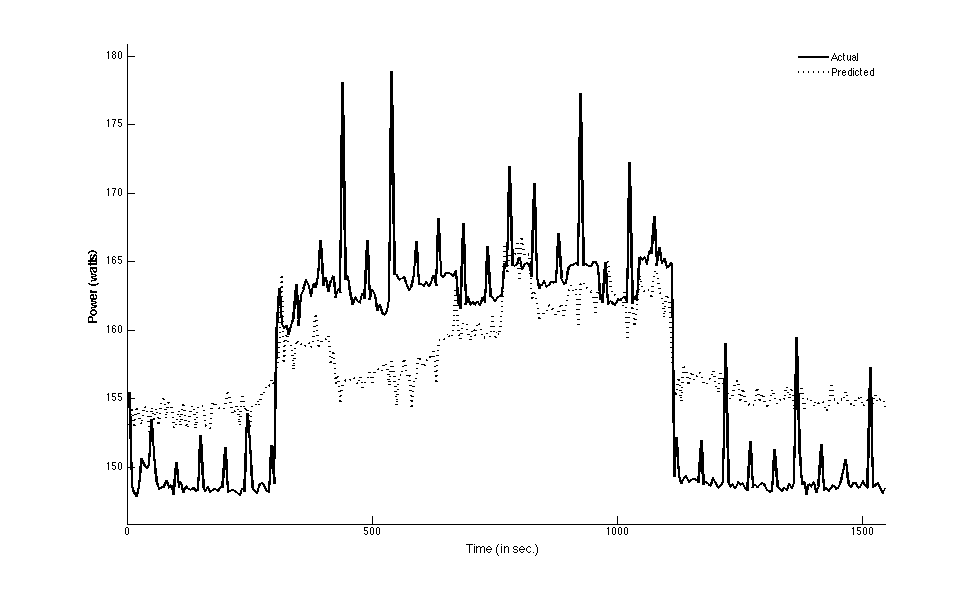
\includegraphics[width=0.5\linewidth,height=2in]{allpower/amd_ar_astar}
  }
  \subfloat[Astar/Intel.]{%
    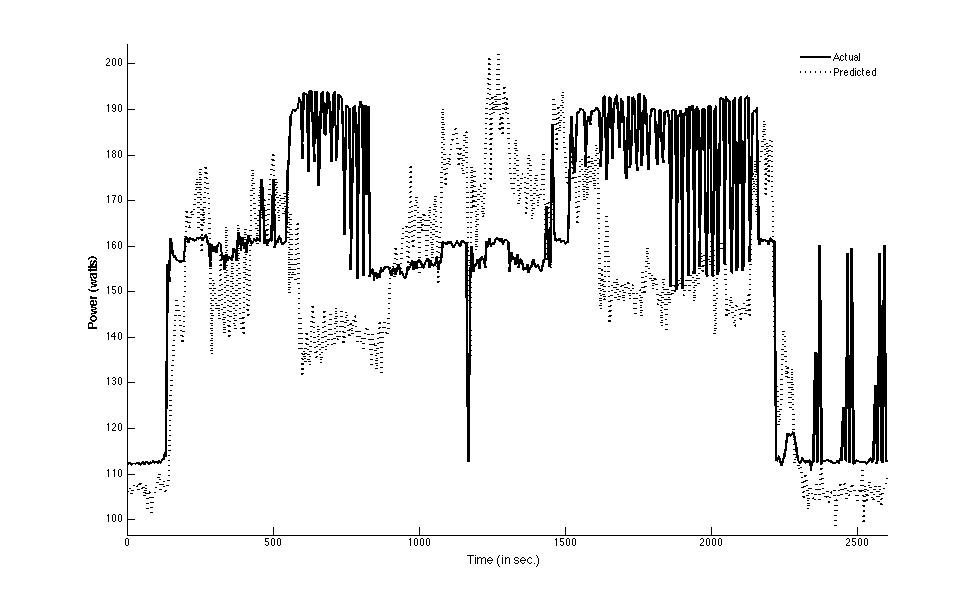
\includegraphics[width=0.5\linewidth,height=2in]{allpower/intel_ar_astar}
  }\\
  \subfloat[Zeusmp/AMD.]{%
    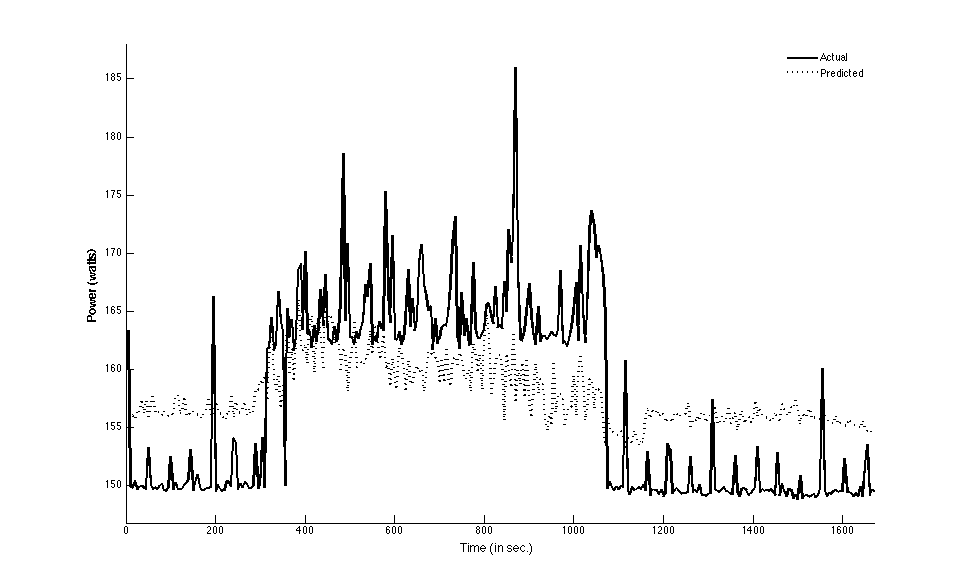
\includegraphics[width=0.5\linewidth,height=2in]{allpower/amd_ar_zeusmp}
  }
  \subfloat[Zeusmp/Intel.]{%
    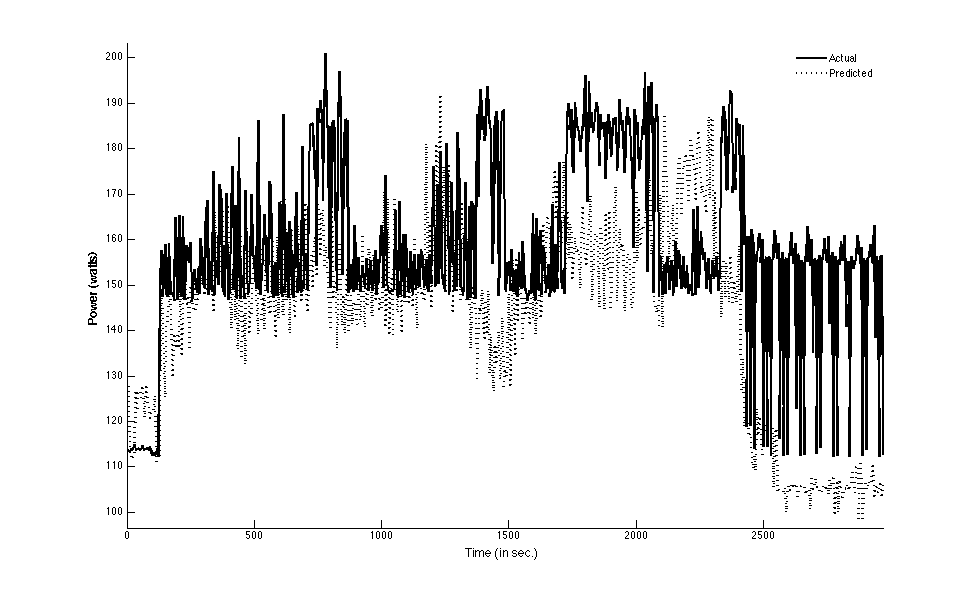
\includegraphics[width=0.5\linewidth,height=2in]{allpower/intel_ar_zeusmp}
  }
  \caption{Actual power results versus AR(1) predicted results for AMD Opteron
    and Intel processors.}
  \label{fig:comparear}
\end{figure}
Consider the traces of actual power shown in
\figurename~\ref{fig:comparear} SPEC CPU2006 \texttt{astar} and
\texttt{zeusmp} benchmark as executed on an AMD Opteron or Intel Nehalem
server.  We saw indications of (1) periodic behavior and (2) large
swings in the power draw throughout the course of the benchmark run.
Similar scenarios were observed for other benchmarks on the AMD Opteron
server and the Intel Nehalem server under this work.  Linear
regression-based prediction for power draw can mis-predict substantially
(up to 44\%, as indicated in Table~\ref{tab:modelerroroptIntel}).  Thus,
it is reasonably conjectured that \textit{non-linear dynamics} do exist
in server systems.  Given large swings in power draw usually occur to a
typical server and cannot be completely attributed to noise, more
accurate prediction than linear auto-regression and MARS
\cite{Friedman1991} is indispensable.

\section{Chaotic prediction}
\label{sec:chaospredict}
The continuous systems expressed in \equationname~\eqref{eq:linmodel},
\eqref{eq:tea}, and \eqref{eq:thermcost} can
be viewed as a multi-variate differential equations in the time domain
(energy being power used in a time period).  The time series
approximation of a system solution can be viewed as a projection of
the flow of \equationname~(\ref{eq:linmodel}) onto a surface~\cite{Liu2010}.
The projection is defined in a way that the behavior (i.e., energy consumption)
of the dynamic system is reflected in our discrete approximation
(i.e., our time series measures).

We performed an analysis on the data collected from our test systems to
determine if the behavior of our time series can be attributed to some
form of chaotic behavior.  A chaotic process is one which is highly
sensitive to a set of initial conditions.  Small differences in those
initial conditions yield widely diverging outcomes in such chaotic
systems.  In order to determine whether a process is chaotic, we must be
able to show that (1) it demonstrates high sensitivity to initial
conditions and topological mixing, and (2) its periodic orbits are dense
\cite{Sprott2003}.  After analyzing our experimental data, we believe
that the power consumption of a server demonstrates \textit{chaotic behavior}.

In order to evaluate a server's sensitivity to initial conditions, we
consider the Lyapunov exponents of the time series data observed while
running those benchmarks described in the previous section.  The
Lyapunov exponent quantifies the sensitivity of a system such that a
positive Lyapunov exponent indicates that the system is chaotic
\cite{Sprott2003}.  The average Lyapunov exponent can be calculated using
$\lambda = \lim_{N\to\infty}\frac{1}{N}\sum_{n=0}^{N-1}ln|f'(X_n)|$.

We found a positive Lyapunov exponent when performing this calculation
on our data set, ranging from 0.01 to 0.28 (or 0.03 to 0.35) on the AMD
(or Intel) test server, as listed in Table~\ref{tab:chaotic}, where
each pair indicates the parameter value of the AMD server followed by
that of the Intel server.  Therefore, our data has met the first and
the most significant criterion to qualify as a chaotic process.

The second indication of the chaotic behavior of the time series in
\equationname~\eqref{eq:tseries} is an estimate of the Hurst parameter
$H$ for the data sets collected in each benchmark.  A real number in the
range of $(0, 1)$, the Hurst parameter is in the exponents of the
covariance equation for Fractional Brown motion (fBm) \cite{Sprott2003}.
If the value of the Hurst parameter is greater than $0.5$, an increment
in the random process is positively correlated and long range dependence
exists in the case of time series.  In a chaotic system, a value of $H$
approaching 1.0 indicates the presence of self-similarity in the system.
As demonstrated in Table~~\ref{tab:chaotic}, the time series data
collected in our experiments all have values of $H$ close to 1.0,
ranging from 0.93 to 0.98 (or 0.93 to 0.97) on the AMD (or Intel) test
server.
  \begin{table}[t!]
    \caption{Indications of chaotic behavior in power time series (AMD, Intel)}
    \label{tab:chaotic}  
    \centering
    \begin{tabular}{c  r r r }
      \hline
      \multicolumn{1}{c }{\textbf{Benchmark}}&\multicolumn{1}{c}{\textbf{Hurst}}&&\multicolumn{1}{c}{\textbf{Average}}\\
      \multicolumn{1}{c }{~}&\multicolumn{1}{c}{\textbf{Parameter}}&&\multicolumn{1}{c}{\textbf{Lyapunov}}\\
      \multicolumn{1}{c }{~}&\multicolumn{1}{c}{($H$)}&&\multicolumn{1}{c}{\textbf{Exponent}}\\
      \hline
      bzip2    &(0.96, 0.93)&&(0.28, 0.35)\\
      cactusadm&(0.95, 0.97)&&(0.01, 0.04)\\
      gromac   &(0.94, 0.95)&&(0.02, 0.03)\\
      leslie3d &(0.93, 0.94)&&(0.05, 0.11)\\
      omnetpp  &(0.96, 0.97)&&(0.05, 0.06)\\
      perlbench&(0.98, 0.95)&&(0.06, 0.04)\\
      \hline
    \end{tabular}
\end{table}

In the thermal domain, a study of the time-series observations of core
die temperatures for the Intel processor in our evaluation indicates the
presence of chaotic behavior for the thermal domain as well as the power
domain.    As demonstrated in
Table~~\ref{tab:chaotictemp}, the time series data collected in our
experiments all have $H$ values close to 1.0, ranging from 0.95 to 0.99
for the Intel server in our test environment.

\begin{table}[tbhp]
\caption{Chaotic behavior in core die temperature time series}
\label{tab:chaotictemp} 
\centering 
\begin{tabular}{lcc}
\hline
\hline
 & Hurst exp. ($H$) & Lyaponov exp. ($\lambda$) \\
\hline
Core 0 & 0.99 & 0.051 \\
Core 1 & 0.98 & 0.019 \\
Core 2 & 0.97 & 0.034 \\
Core 3 & 0.95 & 0.040 \\
\hline
\end{tabular}
\end{table} 

From a predictive standpoint, the unpredictable deterministic behavior
of chaotic time series means that it is difficult to build a predictor
that takes a global parametric view of the data in the series.  However,
it is possible to generate a highly accurate short-term prediction by
reconstructing the attractor in the phase space of the time series and
applying a form of least square prediction to the resulting vector space
\cite{Itoh1995,Su2010}.

\subsection{Chaotic Attractor Predictors}
\label{sec:capps}
With the time series introduced in \equationname~\eqref{eq:tseries}, let $y_{t}$ be
the value of $E_{system}$ at time $t$, $r$ be the total number of PeCs and
performance measures to provide metric readings,
and $X_{t}$ be the vector of those $r$ metric readings at time $t$.
According to Taken's Delay Embedding Theorem \cite{Sprott2003},
there exists a function $\hat{f}(X_{t})$ whose behavior in the phase
space reflects the behavior of the attractors in the original time
series values $y_{t}$.
Consequently, for given $\hat{f}$, a known $X_{t}$ reveals system energy
consumption at time $t$, namely, $y_{t}$.
If $X_{t}$ can be predicted accurately for future time $t$
(likely based on past metric readings), system energy consumption
at future $t$ can be estimated properly.
To this end, it is necessary to find a means for approximating $\hat{f}$.

We introduce the concept of Chaotic Attractor Prediction (CAP) that
defines $\hat{f}$ in terms of least squares regression of a
multivariate local polynomial of degree $r$.  Multivariate local 
regression is a common non-parametric technique for time series
approximations.  With CAP, we extend this concept to predict the
behavior of a chaotic time series by following the approximation method
to take advantage of its polynomial time complexity while capturing the behavior
dynamics of testing systems.

Let $X$ be an observation (involving $r$ measures of 
\begin{equation*}
MP(t+\Delta t) =[MP_{proc},MP_{mem}, MP_{hdd}, MP_{board}, MP_{em}]^{T}
\end{equation*}
for a given server, as described earlier) at some future time $t+\Delta
t$ and $X_{u}$ be a prior observation (involving $r$ metric readings of
$MP(u)$) at time $u$ for $u=t-1, t-2, \dots, t-p$.  CAP localizes and
addresses the possibility of noise in our observations through
\textit{kernel weighting}.  This process starts with the standard
multivariate normal density function of $K(x)$ =
$(2\pi)^{-\frac{m}{2}}exp(-\|X\|^{2}/2)$ (where $\|X\|$ is the norm of
vector $X$) for smoothing out values of a local neighborhood, over which
our CAP is defined.  Let the bandwidth of $\beta$ be a non-negative
number and $K_{\beta}(X)$ equal $K(X/\beta)/\beta$~\cite{Fan1996}.  The
function of $K_{\beta}$ serves as a \textit{kernel} to smooth out noise
in our original observations in a non-parametric manner.  It has been
shown that $\beta$ determines the degree of smoothing produced by the
kernel~\cite{Fan2005}.  Selection of a small $\beta$ value does not
adequately address issues of noise, while a too large $\beta$ value
results in excessive bias in the results and may hide important dynamics
of the underlying function $\hat{f}$~\cite{Turlach1993}.  A preferred
choice for $\beta$ can be computed by: $\beta =
\left(\frac{4}{3p}\right)^{\frac{1}{5}}\sigma$, where $\sigma$ is the
standard deviation of observed values, estimated via the formula of
$\bar{\sigma}$ = $median(|x_{i}-\bar{\mu}|)/0.6745$, with $\bar{\mu}$
being the median of observed values ~\cite{Bowman1997}.
 
An approximation for $\hat{f}$ is defined subsequently in terms of
a locally weighted average \cite{Box1994,Fan1996} over the next
$n$ observations, based on the prior $p$ observations of $X_{t-1},
\ldots, X_{u}, \ldots, X_{t-p}$ (each with $r$ measures, namely,
$MP(u) = \left[MP_{proc}, MP_{mem}, MP_{hdd}, MP_{board}, MP_{em}\right]^{T}$,
as described earlier):
  \begin{equation}
    \label{eq:localconst}
    \hat{f}(X)=\dfrac{\displaystyle\sum_{d=t}^{t+n-1}O_{p}*K_{\beta}(X_{d}-X)}{\displaystyle\sum_{d=t}^{t+n-1}K_{\beta}(X_{d}-X)}\nonumber
  \end{equation}
with $O_{p}=(X_{t-1}, X_{t-2}, \ldots, X_{t-p})$.
 
The process can be improved by defining a local approximation
via applying a truncated Taylor series expansion of $\hat{f}(X)$ for $X$ at nearby $x$:

  \begin{equation}
    \label{eq:localtaylor}
    \hat{f}(X)=\hat{f}(x)+\hat{f}^{'}(x)^{T}(X-x).\nonumber
  \end{equation}

The coefficients of the polynomial $\hat{f}$ are then determined by minimizing
  \begin{equation}
    \label{eq:lsq}
    \displaystyle\sum_{d=t}^{t+n-1}\left(X_{d}-a-b^{T}(X_{d}-x)\right)^{2}*K_{\beta}(X_{d}-x).
  \end{equation}
 with respect to $a$ and $b$, which are estimators to
$\hat{f}(x)$ and $\hat{f}'(x)$, respectively.  The predictor generated
by solving \equationname~\eqref{eq:lsq} can be explicitly written, according to
\cite{Box1994}, as
  \begin{equation}
    \label{eq:locallin}
    \hat{f}(x)=\frac{1}{n}\displaystyle\sum_{d=t}^{t+n-1}(s_{2}-s_{1}*(x-X_{d}))^{2}* K_{\beta}((x-X_{d})/\beta)
  \end{equation}
with $s_{i}=\frac{1}{n}\displaystyle\sum_{d=t}^{t+n-1}(x-X_{d})^{i}*K_{\beta}((x-X_{d})/\beta)$, for $i$ = 1 or 2.
\subsection{CAP Creation}
\label{sec:cappcreate}
There are three steps involved in the process of creating a CAP predictor:
(1) creating a training set for the process, (2) using the
observations from the training set to find the appropriate delay
embedding using Takens Theorem and then apply the nearest neighbors
algorithm in the embedded set to identify the attractors, and (3)
solving the resulting linear least squares problem that arises from
applying \equationname~\eqref{eq:lsq} to the attractors using the
function expressed by \equationname~\eqref{eq:locallin}.

\begin{table}[t!]
  \centering
  \caption{SPEC CPU2006 benchmarks used for model calibration}
  \label{tab:specbenchs}
  \begin{tabular}{c c p{5cm}}
    \hline
    \multicolumn{3}{l}{\textbf{Integer Benchmarks}} \\
    \hline
    bzip2&C&Compression\\
    mcf&C&Combinatorial Optimization\\
    omnetpp&C++&Discrete Event Simulation\\
    \multicolumn{3}{l}{\textbf{FP Benchmarks}} \\
    \hline
    gromacs&C/F90&Biochemistry/Molecular Dynamics\\
    cacstusADM&C/F90&Physics/General Relativity\\
    leslie3d&F90&Fluid Dynamics\\
    lbm&C&Fluid Dynamics\\
    \hline
  \end{tabular}
\end{table}
The training set for the predictor is constructed from a consolidated
time series created by executing the SPEC CPU2006~\cite{Henning2006}
benchmarks listed in Table~\ref{tab:specbenchs} on target systems.  The
benchmarks were selected using two criteria: sufficient coverage of the
functional units in the processor and reasonable applicability to the
problem space.  Components of the processor affect the thermal envelope
in different ways~\cite{Kumar2008}.  This issue is addressed by
balancing the benchmark selection between integer and floating point
benchmarks in the SPEC CPU2006 benchmark suite.  Second, the benchmarks
were selected from the suite based upon fit into the problem space.
Each benchmark represents an application typical of the problems solved
on high-performance application servers.  

Each benchmark in the calibration set was executed with a sampling
interval of $t=5$ seconds.  The observations from each time interval
were consolidated on this time interval using two methods: arithmetic
mean (average) and geometric mean.  Trial models were constructed using
each method and a statistical analysis of variance indicated that time
series generated from the geometric mean
produced the best fit to the collected data.
   
\subsection{Time Complexity}  
The time complexity of creating a predictor is governed by the third
step in the process.  The task of reconstructing the state space by
delay embedding is linear in time as one must make up to $d$ passes
through the observations, under the embedding dimension of $d$.
Thus, the time required is $O(dn)$, where $n$ is the number of future
observations.  Then, it becomes a matter of applying a naive form of
$k^{th}$ nearest neighbors algorithm to identify the points in the
attractors.  This step involves finding the squared distance of all the
points in the nearest analogs in the Takens set and then sorting the
result to determine the $d$-nearest neighbors.  This step takes
$O(n\log{n}+n)$.  The high cost of computing the linear least squares
solution in the third step is avoided by using the explicit expression
given in \equationname~\eqref{eq:locallin}.  The time complexity of computing this
expression can be shown to be $O(n*n)$, with $O(n)$ due to computing
$s_{i}$, for $i$ = 1 or 2.  As a result, the time complexity for
establishing a CAP predictor equals $O(n^{2})$.  It should be noted that
the construction of a CAP predictor is done only once for a given
server, irrespective of applications executed on the server.  Such
construction is based on past PeC observations (totally, $p$ of them)
to predict the future PeC readings.  As $p$ grows (with more past PeC
observations involved), the time complexity of CAP increases linearly,
as can be obtained in \equationname~\eqref{eq:lsq}.  The actual computation time
results under different $n$ and $p$ values for our CAP code implemented
using MATLAB are provided in the next section.
\begin{figure}[tp]
    \centering
    %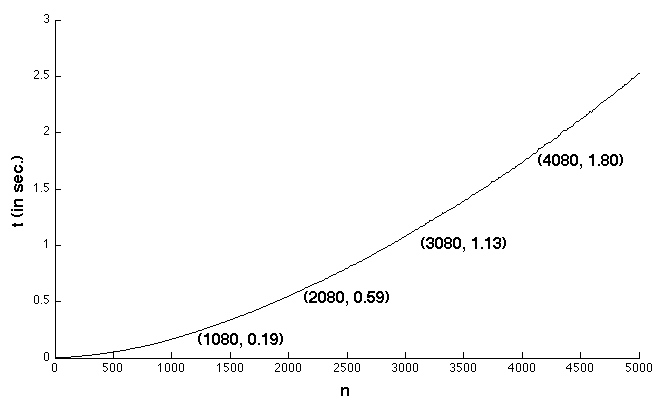
\includegraphics[scale=0.6]{complexity}
    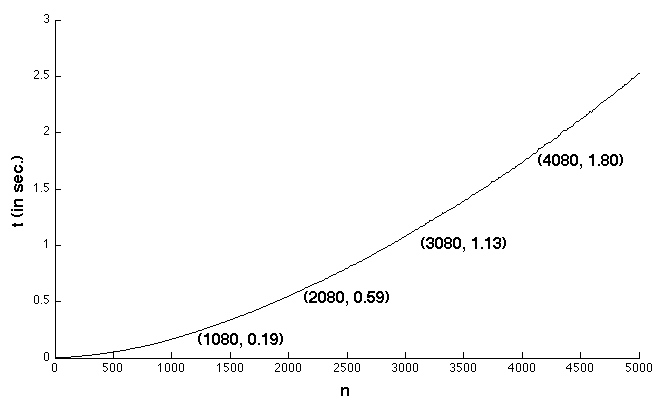
\includegraphics[width=0.9\linewidth,height=2.5in]{complexity}
    \caption{CAP time complexity versus no. of future observations.}
    \label{fig:complexity}
\end{figure}
\hspace{0.3cm}
\begin{figure}
    \centering
%    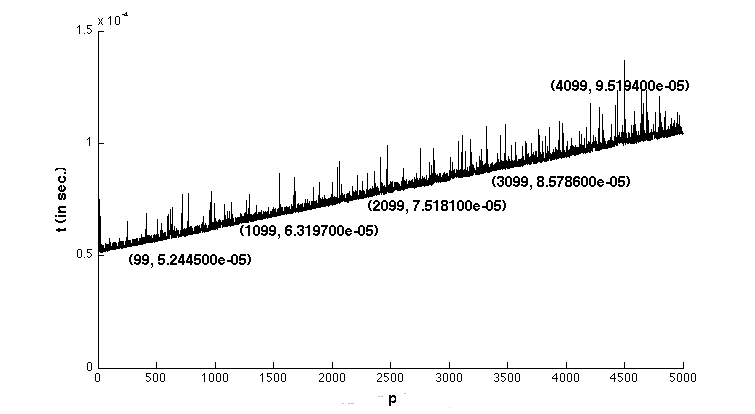
\includegraphics[scale=0.6]{complexity_p}
    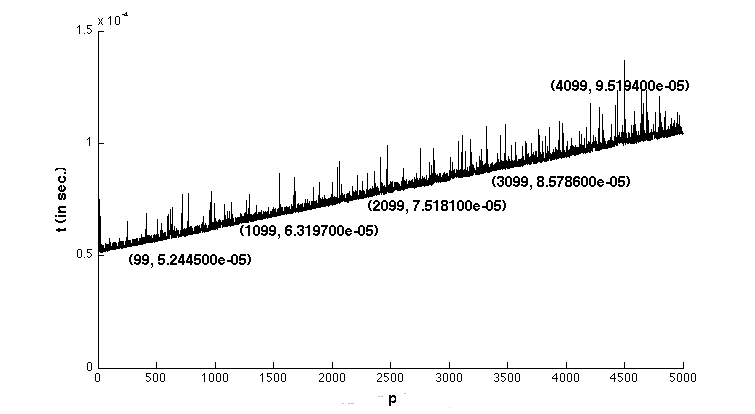
\includegraphics[width=1.0\linewidth,height=2.5in]{complexity_p}
    \caption{CAP time complexity versus no. of past observations.}
    \label{fig:complexityp}
\end{figure}

\section{Thermal Chaotic Attractor Predictors}
\label{sec:therm-chaot-attr} 
We use the measured PeCs listed in Table~\ref{tab:intelmodel} to
estimate the quantities of $\Theta(A, D_{A}, t)$ and $E_{A}(A, D_{A},
t)$ in \equationname~\eqref{eq:thermcost}.  Specifically, thread length
is estimated in each time period by the PeC measure of $IR$, namely, the
total number of instructions retired during that thread execution.  The
total data amount associated with thread execution is measured by
summing up (1) the data bytes moved across the QuickPath links on the
processor (reflected by $QPL_{C}$ and $QPL_{IO}$), (2) last-level cache
misses ($CM_{i}$, $1\leq i \leq 4$), and (3) data read from or written
to disks.  as listed under the contributor of "application data set" in
Table~\ref{tab:intelmodel}.  System temperature is measured using the
ambient temperatures reported by the system, as listed under the
contributor of "system temperature."

\subsection{Thermal CAP Creation}
\label{sec:therm-calibrate}
We establish our thermal CAPs using two applications that are expected
to yield the extreme thermal results for training execution: the idle
scenario and the most stress scenario.  An idle application referred to
no application thread ready for execution and thus the testbed runs only
the OS threads, whereas the most stress application leads to the highest
processor utilization coupled with heaviest memory activities, achieved
by launching multiple instances of the FreeBSD \texttt{cpuburn} stress
testing codes for concurrent execution, one per core with symmetric
multiple threads disabled.  The \texttt{cpuburn} stress test code
implements a single-threaded infinite loop with a sequence of integer
and floating-point operations and large blocks of memory reads and
writes to thermally stress the testbed system, driving it close to a
thermal emergency.  The use of these two extreme thermal scenarios is
preferred over employing SPEC CPU2006 benchmarks for tCAP establishment,
since any typical application execution will lies between the two
extremes, as far as the coefficients of tCAP are concerned.

These two training scenarios run for 600 seconds, with PeCs sampled at
an interval of $t=5$ seconds for establishing tCAP.  The procedure for
establishing tCAP is the same as what was described earlier
\cite{Lewis2010}, and it involved three steps. First, the training set
is constructed by consolidating the observed PeCs into a time series
using geometric means.  In the second step, the Takens Embedding
Theorem~\cite{Su2010} is applied to find delay embedding, with the
nearest neighbors algorithm then employed to identify the set of
attractors using the embedded set.  Finally, our tCAP is established by
solving the linear least squares problem resulted from fitting a
multi-variate polynomial to the attractor set.  The time complexity of
establishing tCAP equals O($n ^2$), where $n$ is the number of sampled
PeCs~\cite{Lewis2010}.  Note that the establishment of the attractor set
for tCAP is required only once for a processor type, irrespective of
applications executed on the processor.

% Following comment block used by GNU-EMACS and AUCTEX packages
% Please do not remove.
%%% Local Variables: 
%%% mode: latex
%%% TeX-master: "dissertation.tex"
%%% TeX-PDF-mode: t
%%% TeX-source-correlate-mode: t
%%% End: 
